%!TEX root = thesis.tex


\chapter{Causal Inference for Recommendation}

We develop a causal inference approach to recommender systems.
Observational recommendation data contains two sources of
  information: which items each user decided to look at and which of
  those items each user liked.  We assume these two types of
  information come from different models---the \textit{exposure} data
  comes from a model by which users discover items to consider; the
  \textit{click} data comes from a model by which users decide which
  items they like.  Traditionally, recommender systems use the
  click data alone (or ratings data) to infer the user preferences.
  But this inference is biased by the exposure data, i.e., that users
  do not consider each item independently at random.  We use causal
  inference to correct for this bias. On real-world data, we
  demonstrate that causal inference for recommender systems leads
  to improved generalization to new data.


\section{Introduction}

The goal of recommender systems is to infer users' preferences for
items and then to predict items that users will like. We develop a
causal inference approach to this problem.

Here is the idea. Observational recommendation data contains two
sources of information: which items each user decided to look at and
which of those items each user liked. For example, one of the data
sets we analyze contains which movies each user watched and which of
them each liked; another contains which scientific abstracts each user
saw and which PDFs each decided to download.

We assume these two types of information come from different
models---the \textit{exposure} data comes from a model by which users
discover items to consider; the \textit{click} data comes from a model
by which users decide which items they like. Traditionally,
recommender systems use the click data alone (or ratings data) to
infer the user preferences. But this inference is biased by the
exposure data, i.e., that users do not consider each item
independently at random.

We use causal inference to correct for this bias. First, we estimate
the exposure model from the exposure data, a model of which items each
user is likely to consider. Then we fit the preferences with weighted
click data, where each click (or skip) is weighted by the inverse
probability of exposure (from the exposure model). This is a
propensity weighting approach to causal
inference~\citep{imbens2015causal}, i.e., we warp the observational
click data as though it came from an ``experiment'' where users are
randomly shown items. We study several variants of this strategy.

Why might this work?  Consider the film enthusiast (from our data) who
mostly watches popular drama but has also enjoyed a couple of
documentaries (``Crumb'' and ``The Cruise'').  A classical
recommendation system will infer film preferences that center around
drama.  Our causal method detects a preference for drama too, but
further up-weights the preference for documentaries. The reason is
that the history of the user indicates that she is unlikely to have
been exposed to many documentaries; the method values its signal from
the two she did like.  Consequently, when we recommend from among the
unwatched films, our method promotes documentaries (``Fast, Cheap \&
Out of Control'' and ``Paris Is Burning'') that the user (in held-out
data) also liked.  Across users, on real-world data, we demonstrate
that causal inference for recommender systems leads to improved
generalization to new data.



\parhead{Related work.} \citet{Marlin09NMAR} first formalized
statistical models for correcting rating-selection bias. They posit
that a user's decision to rate an item depends on the user's opinion
of the item. They propose a mechanism to correct for this self-selection
bias, based first on generating a rating and then conditionally on
whether the rating is observed. Others have proposed different rating
models using this same mechanism
\cite{ling12response,HernandezLobato14nmar}. In contrast, our model
(similar to \citep{Liang16exposure}) first generates each user's
exposure to an item and then her rating. Unlike
\citep{Liang16exposure}, we work with explicit click data. Thus we can
use causal inference to de-bias the resulting inference of user
preferences.

% Their hypothesis is validated with an experiment
% \cite{DBLP:conf/uai/MarlinZRS07}: they observe that the distribution
% of ratings for randomly-selected items differs from the ratings of
% user-selected items (we fit these data with our model in
% \Cref{sec:empirical_study}). In particular users favor rating items
% they have a high opinion of.

%As such unobserved ratings are not missing at random (MAR). Modeling
%ratings as being missing at random thus yields biased models. 

% Also, this line of work is rooted in the theory of missing
% data~\cite{little1986statistical} and does not appeal to causal
% inference. As a result concepts such as inverse propensity weighting
% do not have direct equivalents in their work.

Solving recommendations using causality has been explored in the
multi-arm bandit literature (e.g.,
\cite{li2010contextual,vanchinathan14explore,zhao13interactive,li15counterfactual}).
They focus on unbiased evaluation of a recommendation policy, though
using biased data (e.g., data collected in web log). This work
typically uses importance sampling, weighting the probability of each
observed click under the logging policy and under the (new)
recommendation policy. We use the same tools for data
re-weighting---propensity score weighting is equivalent to importance
sampling---but we reason about preferences rather than recommendation
policies. Further we work in a batch learning setting (as opposed to
online learning).

% [todo] above, i didn't find the "preferences versus policy" argument
% too convincing.  user preferences are simply parameters to the
% per-user recommendation policy.  can we say something different? -dmb

The recent work of \citet{schnabel16treatment} is closest to ours. The
authors propose a causal inference approach to learning unbiased
estimators from biased rating data. One important difference with our
work is that their propensity weights depend on user preferences
(either directly through ratings or indirectly through user and item
covariates)---a process known as self-selection---rather than
reflecting exposure, as in our work. Their formalization of the
problem also differs: they appeal to empirical risk minimization while
we take a Bayesian perspective.

% [xxxx] below, i didn't understand this.

% As a concrete example, the Bayesian perspective frames conditional and
% marginal predictions.

%%% Local Variables:
%%% mode: latex
%%% TeX-master: "causal_rec_nips"
%%% End:


%!TEX root = causal_rec_nips.tex

\section{A causal model for recommendation}

In this section we develop our method.  We describe explicit
recommendation data, a joint model of exposure and clicks, how we do
prediction, and how we do causal inference.

\parhead{Data.}  Our data are \textit{explicit data}: we know which
items each user saw and which of those items each clicked (liked) or
skipped (disliked). For example, in \Cref{sec:study} we analyze a large
collection of click data from
arXiv.org.\footnote{\url{http://arxiv.org} is a pre-print repository
  for scientific papers.} We know which arXiv abstracts a user has
viewed and, among those, which PDFs she has downloaded.  Our goal is
to infer each user's latent preferences for items and then to use
those preferences in a recommendation system.

We begin with notation for the data.  A user is indexed by $u$ and an
item is indexed by $i$.  There are two types of observations.  The
\textit{exposure data} is $a_{ui}$, whether user $u$ had the
opportunity to click on item $i$.  (We use the verb ``click'' for
concreteness; this can be any type of interaction, including
``download,'' ``purchase,'' ``listen,'' or ``watch.'') The
\textit{click data} is $y_{ui}$, an indicator of whether user $u$
clicked on item $i$ (liked) or decided to skip the item (disliked).

These data capture the users' clicks.  There are some items which a
user was exposed to ($a_{ui} = 1$) but did not click on
($y_{ui} = 0$); there are other items that a user was exposed to
($a_{ui} = 1$) and did click on ($y_{ui} = 1$); finally, there are
items that a user was not exposed to ($a_{ui}=0$) and, by definition,
did not click on ($y_{ui} = 0$).  A user cannot click on an item she
is not exposed to.

\parhead{Joint models of exposure and clicks.}  We build a joint model
of this data: an exposure model of what the user sees and a click
model of what the user clicks on, conditional on her seeing it.  The
key idea behind our approach is this.  Given observational data, i.e.,
data collected by users exploring information and clicking on items,
classical inference of the click model---of the user's preferences for
clicking on items that she is exposed to---is incorrect because of the
biases induced by the exposure model.  We take a causal inference
approach to this problem: we infer the user's preferences from an
imagined experiment where each item is exposed with equal probability.

We first describe the \textit{observation joint}, from which we
observe our data set.
\begin{align*}
  a_{ui} & \sim f(\cdot \g \pi_{ui}) \\
  y_{ui} \g a_{ui}=0 & \sim \delta_{0}(\cdot) \\
  y_{ui} \g a_{ui}=1 & \sim g(\cdot \g \mu_{ui}).
\end{align*}

Here the exposure and click models are generic.  Each is governed by
the exposure parameter $\pi_{ui}$ and click parameter $\mu_{ui}$,
respectively.

For example, one exposure model we study is a Bernoulli with an
item-specific parameter.  We call this the popularity exposure because
it allows some items to be more likely to be exposed (across users)
than others,
\begin{align}
\kern-1em a_{ui} &\sim \Bern(\rho_i). & \qquad\qquad\qquad\qquad\qquad\qquad\textit{(Popularity exposure)} &
  \label{eq:popularity}
\end{align}

Alternatively, the exposure model can capture a user's preferences for
seeking out items.  We will also study Poisson factorization,
\begin{align}
  \kern-1em a_{ui} &\sim \textrm{Poisson}(\pi_u^\top \gamma_i),
  & \qquad\qquad\qquad\qquad\textit{(Poisson factorization exposure)}&
  \label{eq:poisson-factorization}
\end{align} which finds
non-negative embeddings for users and
items~\citep{Gopalan:2015}.\footnote{Though Poisson models capture
  count data, they are effective for binary data with many
  items~\citep{Gopalan:2015}.}

For the click model, we use classical probabilistic matrix
factorization~\citep{mnih2007probabilistic}.  Conditional on being
exposed, the click comes from a normal distribution,
$y_{ui} \g a_{ui} = 1 \sim \cN(\theta_u^\top \beta_i,
\lambda_y^{-1})$.
Here $\theta_u$ is a latent $K$-vector of user preferences and
$\beta_i$ is a latent $K$-vector of item attributes. In all models,
the conditional distribution of a click $y_{ui}$ given that a user is
not exposed to the item ($a_{ui} = 0$) is a point mass at zero.

% [todo] above, we need to justify using a normal for zero-one data.
% i think i should finally write that appendix about the poisson
% versus the normal.

\parhead{Forming predictions.}  Our goal is to use this model to form
future predictions about the users.  We are given observed data
$\cD = \{(a_{ui}, y_{ui})\}$ of what each user was exposed to and
what each user clicked on.  We want to predict what we should expose
them to in the future, i.e., what they would like to see.

We will study two ways of predicting. One is to form conditional
predictions as the probability that a user clicks on an item given
that she is exposed to it,
\begin{align}
  &\E{y_{ui} \g a_{ui} = 1, \cD}.  &\quad\quad\quad\quad\quad\quad\quad\quad\quad\quad\quad\quad\textit{(Conditional prediction)}&
  \label{eq:conditional-prediction}
\end{align}
Alternatively, we use marginal predictions, where we marginalize out
the exposure variable
\begin{align}
  &\E{y_{ui} \g \cD} = p(a_{ui} \g \mu_{ui}, \cD) \E{y_{ui} \g a_{ui} =
  1, \cD}. & \textit{(Marginal prediction)}&
  \label{eq:marginal_preds}
\end{align}
The marginal prediction uses that $y_{ui} = 0$ when $a_{ui} = 0$.  It
is apt when the exposure model also contains information about the
user, i.e., information about what the user is likely to seek out.

% [xxxx] commented out (for space, and b/c laurent was confused by it)

% It tries to predict items the user will find and like. \todo{LC: I'm
% not sure what we mean here. It sounds like this is useful only in
% certain instances or with certain kinds of data.}

% [xxxx] took this out to be more generic -dmb
% (This does not require forming inferences about the exposure model.)

% [!!!] consider moving prediction after inference -dmb

Note that these methods require approximating the posterior predictive
distribution of $y_{ui}$ and $a_{ui}$ given the data.  We now turn to
this inference problem.

% [xxxx] cutting room floor -dmb

% The common practice is to ignore exposure and infer the governing
% parameters of the click model, i.e., the users' preferences and
% items' attributes.  Alternatively, if we include exposure in our
% predictions, we can infer the governing parameters of both models
% and then predict which items a user will be exposed to and click on.

% [todo] i think we can better explain the issue here -dmb

\parhead{Causal inference for recommendation.} One way to solve the
inference problem is with classical Bayesian inference, where we
condition on the observed data and then use posterior prediction to
recommend items.  But there is an issue with using classical Bayesian
inference to form recommendations: the data we observe $\Dobs$ is not
the data from which we would like to infer the user's preferences and
item attributes, i.e., the click model. The reason is that the
exposure model---the distribution that governs what each user
sees---biases our inference about the click model. Items that users
are likely to be exposed exert too much of an influence; items that
users are rarely exposed to have too little influence.

Ideally, we would infer preferences from an experiment, a model that
randomly exposed each user to items and then recorded which items each
one click on.  We call this the \textit{intervention joint},
\begin{align*}
  a_{ui} & \sim \Bern(\pi) \\
  y_{ui} \g a_{ui}=0 & \sim \delta_{0}(\cdot) \\
  y_{ui} \g a_{ui}=1 & \sim g(\cdot \g \mu_{ui}).
\end{align*}
In this model, we have intervened on the mechanism from which users
are exposed to items. (This is the ``mutilated
model''~\citep{pearl2009causality}.) Data from this model leads to
better estimates of the click model (i.e., their preferences) and
better generalization to the items that they will want to click on.

This is a causal approach to the problem.  The observation joint is
the model of how we collected the data; the intervention joint is a
model of a randomized experiment that would (in theory) help us make
the inferences that we need.  The challenge is to use data from the
observation joint to perform inference in the intervention joint.

% [xxxx] removed below; it was repetitive. -dmb

% For concreteness, assume that the click model is the matrix
% factorization model above. We want to use data from the observation
% joint to infer the user preferences $\theta_u$ and item attributes
% $\beta_i$ in the intervention joint.


How do we solve this problem?  Assume for now that the exposure model
is known and is the popularity model, i.e.,
$a_{ui} \sim \Bern(\rho_i)$. We will use \textit{inverse propensity
  weighting}~\citep{imbens2015causal}, which takes samples from the
observation joint and weights them to look like samples from the
intervention joint; this is essentially an importance sampling
technique. Specifically, we weight each observation $(a_{ui}, y_{ui})$
by $1 / \rho_i$ to estimate $\theta_i$. (Because of the click model,
this estimate only relies on those data where $a_{ui} = 1$.) When
inferring a user's preferences, this down-weights the influence of
popular items and up-weights the influence of unpopular items.

More formally, our goal is to obtain a data set
$\mathcal{D} = \{(a_{ui}, y_{ui})\}$ from the intervention joint and
then estimate $p(\theta_u \g \mathcal{D})$. We define the ``do
dataset'' to be the observed data embellished with weights,
$\mathcal{D}^{\textrm{do}} = \{(a_{ui}, y_{ui}, w_{ui})\}$. The
posterior is
\begin{align}
  p(\theta_u \g \mathcal{D}^{\textrm{do}}) \propto
  p(\theta_u) \prod_{i} p(y_{ui} \g a_{ui})^{w_{ui}}
  \label{eq:causal-training}
\end{align}
Intuitively, this assumes that we see each data point ``$w_{ui}$
times'', and that the clicks are conditionally independent given the
preferences.

% [todo] i think the above needs to be more rigorous.  this solves the
% problem of incorporating inverse propensity weighting in bayesian
% inference.

How is this different from standard causality?  One way is that, in
typical causal settings, we have a single causal question \cite{imbens2015causal}.  Here we
have many causal questions (one per item).  What is crucial is that
the causal outcomes are related, each governed by the same set of
parameters.

% [todo] above, this is not rigorous either.  we need to bring out the
% idea that we need IPW even though there is no confounding.  that's
% important.

% [todo] we need to explain the subtle issue of scaling the data and
% making regularizations constant.  maybe this can go in the empirical
% results section.

% [todo] next steps: notice that classical bayesian inference is all
% we need in the exposure model because $a$ blocks $y$.  (i think we
% need some graphical models.)

\parhead{The algorithm.}  We first estimate the exposure model from
the observed data.  This can be the popularity model or Poisson
factorization.  Then, we use the fitted exposure model to weight the
data (by the inverse probability) and fit the click model.  Finally we
use the posterior distribution of the exposure model and (causal)
posterior distribution of the click model to form predictions.  This
procedure generalizes better than Bayesian inference, especially under
intervention, i.e., when we change the distribution of which items a
user is exposed to.

%%% Local Variables:
%%% mode: latex
%%% TeX-master: "causal_rec_nips"
%%% End:


%!TEX root = causal_rec_nips.tex


\section{Empirical study}\label{sec:empirical_study}

We studied causal recommender systems on several data sets. We
compared models trained observationally with models trained causally;
we compared predictions made marginally and those made conditional on
exposure; we studied and evaluated different exposure models, both
those based on popularity and based on personalized preferences; and
we studied typical test sets and test sets that focus on rare
items.\footnote{The source code to reproduce the experimental results
  will be released upon publication.}
% Specifically, we explore the following modeling configurations: a)
% training observationally or causally; b) predicting conditionally or
% causally; c) popularity or personalized exposure model; and d)
% evaluating recommendations by emulating the intervention joint.

We highlight the following results:
\begin{itemize}
\item Poisson factorization (\Cref{eq:poisson-factorization}) is a
  better
  exposure model than the one based on item popularity
  (\Cref{eq:popularity}). We evaluate
  the exposure model both as a standalone model to predict held-out
  exposure and as a component in the whole recommender system.

\item When the test set focuses on rare items, fitting causally
  (\Cref{eq:causal-training})
  gives better generalization than classical inference. Causal
  inference is
  important for generalizing to situations that we do not see in
  training.

\item Accounting for exposure is important when making
  prediction---recommendation with marginal prediction
  (\Cref{eq:marginal_preds}) significantly
  boosts the ranking-based recommendation performance.

\end{itemize}

We give details below. We describe the data, methods, metrics, and
results.

\subsection{Data} \label{sec:data}

We study three types of data (and four data sets):
\begin{itemize}
\item \textit{MovieLens (ML-1M and ML-10M).} User-movie ratings
  collected from a movie recommendation
  service.\footnote{\url{http://grouplens.org/datasets/movielens/}}
  The ratings are on a 1--5 scale.

\item \textit{Yahoo-R3.} Music ratings collected from Yahoo!
  Music services~\cite{Marlin09NMAR}. The ratings are 1--5.

\item \textit{ArXiv.} User-paper clicks from the 2012 log-data of the
  arXiv pre-print server. The data are binarized: multiple clicks by
  the same user on the same paper are considered to be a single click.
  This data contains which papers a user
  downloaded and which she only read the abstract.
\end{itemize}

For ML-1M, ML-10M, and Yahoo-R3, we denote exposure $a_{ui} = 1$ as
user $u$ having rated item $i$. These three datasets are typically
used for rating prediction. Because our end goal is recommendation, we
binarize the ratings and encode preferences as being either positive
or negative ($y_{ui} = 1$ if rating is greater than or equal to 3 and
$y_{ui} = 0$ otherwise). This type of binarization gives better
recommendation performance than directly using predicted
ratings~\cite{hu2008collaborative}.\footnote{We note that
  the Yahoo! data set also contains a random test set, where a subset
  of the users are given 10 randomly selected songs to rate. But most
  of the ratings for this random test set are below 3. Rather,
  we created a skewed test set.}

In ArXiv we denote exposure $a_{ui} = 1$ as user $u$ having viewed the
abstract of paper $i$. Among papers that a user is exposed to, we set
$y_{ui} = 1$ if she downloaded the paper and $y_{ui} = 0$
otherwise.

\begin{table}
\begin{center}
\begin{tabular}{ l c c c c c }
  \toprule
   & \textbf{ML-1M} & \textbf{ML-10M} & \textbf{Yahoo-R3} & \textbf{ArXiv}  \\
  \midrule
  \# of users & 6,040 & 69,878 & 15,400 & 26,541  \\
  \# of items & 3,706 & 10,677 & 1,000 & 80,082 \\
  \# of exposures & 1.0M &  10.0M & 0.3M & 1.9M \\
  \% of exposures & 4.47\% & 1.34\% & 2.02\% & 0.09\% \\
  \bottomrule
\end{tabular}
\end{center}
\caption{Attributes of the data. \# of exposures is the
  number of entries with $a_{ui} = 1$ (rated an item, viewed an abstract). \% of exposure refers to the
  density of the user-item exposure matrix. }
\label{tab:data}
\end{table}

\Cref{tab:data} summarizes the important attributes of these datasets.

\parhead{Data pre-processing.} For each dataset, we create two
training/validation/test splits: regular (REG) and skewed (SKEW). We
create a regular split by randomly selecting the exposed items for
each user into training/validation/test sets, following 70/10/20
proportions. In the regular split, the test set has the same exposure
distribution as the training and validation sets. This is how
researchers typically evaluate recommendation models (with
observational data).

The skewed split rebalances the splits to better approximate an
intervention. We create it by first sampling a test set with roughly
20\% of the total exposures, such that each item has uniform
probability. Training and validation sets are then created from the
remaining data (as in a regular split) with 70/10 proportions. For a
skewed split, the test set will have a completely different exposure
distribution from the training and validation sets. We use this split
to demonstrate that causal inference for recommendation leads to
improved generalization performance.

\Cref{fig:tr_vs_te} shows the scatter plots of the training exposure
distribution (reflected by the empirical item popularity) against the
test exposure distribution on regular and skewed splits of the ML-1M
dataset. The empirical item popularity is computed by counting the
number of users who have been exposed to each item. The skewed split
has a roughly uniform exposure distribution across items, while in the
regular split, both training and test sets follow similar exposure
patterns.

%LC: commented out
%\todo{Part of this paragraph and next one should probably in method section (e.g. MAP estimations, priors on the factors)}

\begin{figure}[!ht]
  \centering
    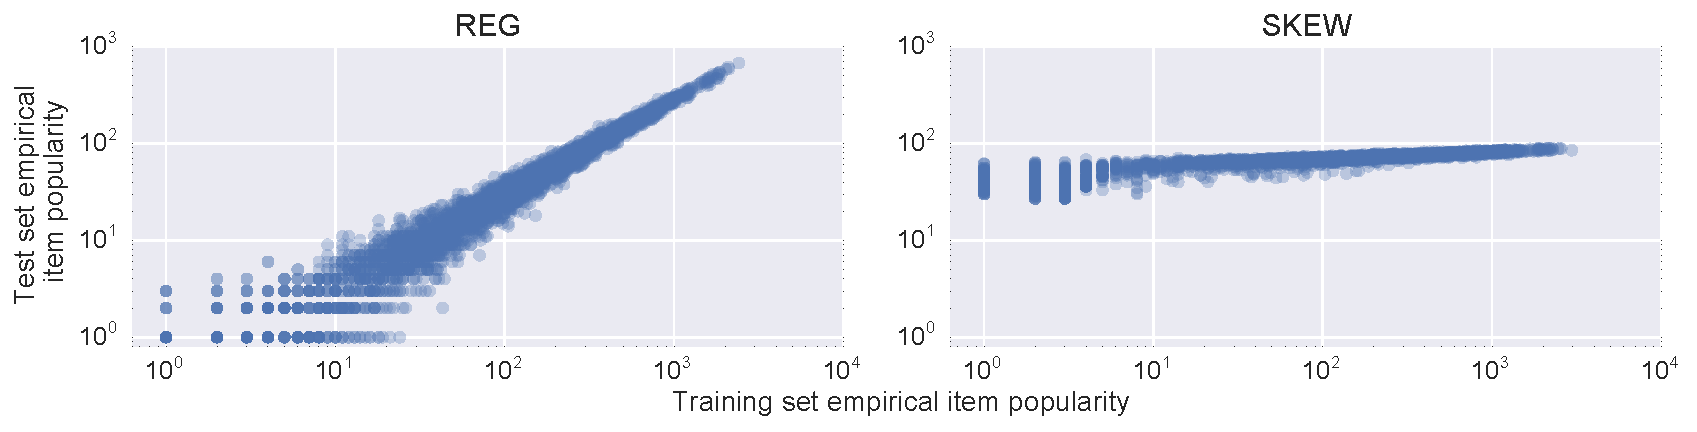
\includegraphics[width=\textwidth]{fig/tr_vs_te}
    \caption{Scatter plots of the training exposure distribution
      (reflected by the empirical item popularity) against the test
      exposure distribution on REG (left) and SKEW (right) splits for
      ML-1M dataset. SKEW split has a roughly uniform exposure
      distribution across items, while in REG split both training and
      test sets follow similar exposure patterns. }
   \label{fig:tr_vs_te}
\end{figure}

\subsection{Methods}

There are several choices in the proposed method.  We explored
combinations of the exposure model, prediction method, and fitting
procedure.  The different choices are summarized below:
\begin{itemize}
\item \textit{Exposure model.\,}
  Popularity (Pop, \Cref{eq:popularity}) or
  Poisson factorization (PF, \Cref{eq:poisson-factorization}).

\item \textit{Prediction.\,} Conditional prediction (Cond, \Cref{eq:conditional-prediction}) or marginal
  prediction (Mar, \Cref{eq:marginal_preds}).

\item \textit{Model fitting.\,} Train the click model causally (CAU,
  \Cref{eq:causal-training}), with inverse propensity weighting, or
  observationally (OBS), with
  classical inference.
\end{itemize}

Among these methods are two baselines. The models that are trained
observationally (OBS) with conditional prediction (Cond) correspond to
classical matrix factorization \cite{mnih2007probabilistic}. The models that
are trained causally (CAU) with conditional prediction (Cond)
correspond to inverse propensity weighted matrix factorization
proposed in \citet{schnabel16treatment}.\footnote{Even though
  \citet{schnabel16treatment} derive the model from empirical risk
  minimization framework, the model objective closely resembles the
  joint log-likelihood of the causally trained model (CAU) with
  conditional prediction (Cond).} We note that this approach
significantly outperformed the previous state-of-the-art model
proposed in \citet{HernandezLobato14nmar} for the task of rating
prediction (though the main focus of this paper is on recommendation).

\parhead{Hyperparameters.} The click model is a matrix factorization.
We place a diagonal normal prior on both user preference
$\theta_u \sim \mathcal{N}(0, \lambda_\theta^{-1} \mathrm{I}_K)$ and
item attributes
$\beta_i \sim \mathcal{N}(0, \lambda_\beta^{-1}\mathrm{I}_K)$. We
perform grid search using
$\lambda_\theta \in \{10^{-4}, 10^{-3}, \dots, 10^4\}$ and
$\lambda_\beta \in \{10^{-4}, 10^{-3}, \dots, 10^4\}$ to select
hyperparameters based on the normalized discounted cumulative gain
(NDCG)~\cite{jarvelin2002cumulated} of the validation set.

We set the dimension of the latent space $K$ to 30. 
%(Increasing $K$ did not lead to validation improvements.) 
To fit the model, we compute the maximum \emph{a posteriori} (MAP)
estimates of the parameters $\theta_u$ and $\beta_i$. This leads to
efficient closed-form coordinates updates, which scale to large
datasets. We use the same random initialization of $\theta_u$ and
$\beta_i$ in all settings. We declare convergence when the mean
squared error on the validation set increases.

\subsection{Metrics}\label{sec:metrics}

We separately evaluate the exposure model, how well we predict which
items a user will see, and the click model, which items a user will
like.  Note that causal inference of the click model uses the exposure
model to compute the propensity score.  Further, marginal prediction
of clicks also uses the exposure model.

We evaluate the exposure model using model fitness to the data
(predictive log-likelihood). We evaluate the click model with
recommendation metrics, both a likelihood-based metric (a tail
probability) and a ranking-based metric (mean average
rank~\cite{charlin2015dynamic}).\footnote{NDCG \cite{jarvelin2002cumulated} is another commonly used
  ranking-based metric. It emphasizes the importance of the top ranks
  by logarithmically discounting ranks. MAR, on the other hand, makes
  no such discounting.} We describe the recommendation metrics in turn.

 % We do not report NDCG because we are more
 %  interested in how different models would rank the relatively rare
 %  items, which are normally far down the list. Both metrics should be
 %  well correlated.}


\parhead{Predictive log tail probability (PLP).} For $y_{ui}$ in the
heldout test set, we compute the predictive log-probability based on
its value and whether we predict conditionally or marginally (see \Cref{eq:marginal_preds}).

Conditional prediction uses
$\mathbb{E}[y_{ui} \mid a_{ui} = 1, \mathcal{D}]$. If $y_{ui} = 1$, we
compute right-tail conditional predictive log-probability for
positively preferred items,
\begin{align*}
  \log \mathbb{P}(y^{\text{pred}}_{ui} > 1 \mid a_{ui} = 1,
  \mathcal{D}).
\end{align*}
Otherwise we compute left-tail conditional predictive
log-probability
\begin{align*}
  \log \mathbb{P}(y^{\text{pred}}_{ui} \leq 0 \mid a_{ui} = 1,
  \mathcal{D}).
\end{align*}
Both correspond to Gaussian tail-probability for matrix factorization.

Marginal prediction uses $\mathbb{E}[y_{ui} \mid \mathcal{D}]$. If
$y_{ui} = 1$, we compute right-tail marginal predictive
log-probability,
\begin{align*}
  \log \mathbb{P}(y^\text{pred}_{ui} > 1 \mid \mathcal{D}) =
  \log\pi_{ui} + \log \mathbb{P}(y^\text{pred} > 1 | a_{ui} = 1,
  \mathcal{D})
\end{align*}
(Recall that $\pi_{ui}$ is the probability that user $u$ is exposed to
item $i$.) Otherwise we compute left-tail marginal predictive
log-probability
  \begin{align*}
    \log \mathbb{P}(y^\text{pred}_{ui} \leq 0 \mid \mathcal{D}) =
    \log\big(\pi_{ui} \mathbb{P}(y^\text{pred}_{ui} \leq 0 \mid a_{ui} =
    1, \mathcal{D}) + (1 - \pi_{ui})\big).
  \end{align*}

The intuition behind PLP is that we would like to have 0's and 1's in
the heldout set well-separated. This is different from the
commonly used metrics for rating prediction, e.g., mean squared error
or mean absolute error, both of which penalize the model unless it
predicts with a perfect 0 and 1. We report average PLP over all the
heldout $y_{ui}$ in the test set.


\parhead{Mean Average Rank.} We compute MAR as follows. For user $u$
we calculate the ranking of all the items $i\in \{1, 2, \dots, I\}$ by
sorting the predictions and excluding the items from the training and
validation sets. Define $\text{rank}(u, i)$ as the predicted rank of
item $i$ for user $u$: $\text{rank}(u, i)=0$ if item $i$ is ranked
first for user $u$ and $\text{rank}(u, i) = I-1$ if ranked last. For
items within a set $I_u$, \begin{align*}
  \text{MAR}_u = \frac{1}{|I_u|}\sum_{i\in I_u} \text{rank}(u, i).
\end{align*}

In our studies, $I_u$ is the item set in the heldout set with
$y_{ui} = 1$, i.e., the items that user $u$ rated positively or the
papers that user $u$ downloaded after looking at the abstract. Since
the value of MAR depends on the size of the item set $I$, we report
the normalized MAR percentile instead as $\text{MAR}_u / I$. This also
corresponds to the expected percentile ranking proposed in
\citet{hu2008collaborative} with binary feedback data. The
interpretation of MAR is on average at what percentile a heldout item
will be ranked (smaller is better). The reported MAR averages over all
users.

\subsection{Results}

We report our studies on all data. We evaluated both the exposure
model alone and the recommender model, which uses the exposure model
to improve its recommendations.

\parhead{Evaluating the exposure model.} We first compare two
different exposure models used in this paper: Poisson factorization
(PF) and the popularity model (Pop). We use the training set
created in \Cref{sec:data} to train the model (for PF, we use
the validation set to monitor convergence). We randomly sample the same
number of entries with $a_{ui} = 0$ as those with $a_{ui} = 1$ and
report the average heldout predictive log-likelihood in
\Cref{tab:eval_expo}.

% [todo] make sure that there are equations for those models and cite
% the equations. -dmb

PF always outperforms Pop. Further, the predictive log-likelihood is
always lower on skewed test sets than on regular test sets. This is
expected because skewed test sets follow a different exposure
distribution from the training and validation sets. This makes it
harder for the exposure model to correctly predict its values.

\begin{table*}
\centering
\begin{tabular}{ c  c c  c c  c c  c c  }
  \toprule
  \multicolumn{1}{c}{} & \multicolumn{2}{c}{\textbf{ML-1M}} & \multicolumn{2}{c}{\textbf{ML-10M}} & \multicolumn{2}{c}{\textbf{Yahoo-R3}} & \multicolumn{2}{c}{\textbf{ArXiv}} \\ \midrule
      & REG & SKEW	 & REG & SKEW     & REG & SKEW          & REG & SKEW  \\ \midrule
  Pop &  -1.39 &  -2.07  & -1.64 &  -2.76 & -1.81 & -2.74       & -3.83 & -3.95 \\
  PF  &  -0.97 &  -1.51  & -1.08 & -2.06 & -1.58 & -2.35        &
                                                                  -2.71 & -2.80 \\
\bottomrule
\end{tabular}
\caption{Heldout predictive log-likelihood for Poisson factorization (PF) exposure model and popularity exposure model (Pop). PF outperforms Pop across datasets. The predictive log-likelihood is generally lower on SKEW than REG. }
\label{tab:eval_expo}
\end{table*}

\parhead{Evaluating the recommender model.} We summarize the log
probability (PLP) and mean average rank (MAR) (described in \Cref{sec:metrics}) in
\Cref{tab:eval_plp} and \Cref{tab:eval_mar}, respectively. The table
reports eight different model configurations based on which
exposure model is used, how the model is fit, and how predictions are
formed.\footnote{There
  are seven distinct
  configurations, as the ones that are trained observationally (OBS)
  with conditional prediction (Cond) will not depend on the exposure
  model. We keep all eight configurations in \Cref{tab:results} for
  easy comparison.} 

\begin{table*}

\begin{subtable}[t]{\textwidth}
\begin{tabular}{ c  c  c  c c  c c  c c  c c  }
  \toprule
  \multicolumn{3}{c}{} & \multicolumn{2}{c}{\textbf{ML-1M}} & \multicolumn{2}{c}{\textbf{ML-10M}} & \multicolumn{2}{c}{\textbf{Yahoo-R3}} & \multicolumn{2}{c}{\textbf{ArXiv}} \\ \midrule
  \multicolumn{2}{c}{} & & REG & SKEW	& REG & SKEW  & REG & SKEW & REG & SKEW  \\ \midrule
  \multirow{4}{*}{Pop} & \multirow{2}{*}{Cond} & OBS & -1.50 & -2.07 & -1.62 & -2.59 & -1.58 & -1.75 & -1.61 & -1.65 \\
  & & CAU & -1.61 & -1.95 & -1.67 & -1.89 & -1.51 & -1.56 & -1.74 & -1.76 \\ \cmidrule{2-11}
  & \multirow{2}{*}{Mar} & OBS & -3.17 & -4.29 & -3.56 & -5.63 & -2.98 & -3.53 & -3.93 & -4.21 \\
  & & CAU & -3.21 & -4.25 & -3.60 & -5.24 & -2.84 & -3.53 & -3.94 & -4.15\\ \midrule
  \multirow{4}{*}{PF} & \multirow{2}{*}{Cond} & OBS & -1.50 & -2.07 & -1.62 & -2.59 & -1.58 & -1.75 & -1.61 & -1.65 \\
  & & CAU & -1.48 & -1.84 & -1.51 & -1.96 & -1.49 & -1.55 & -1.60 & -1.62 \\ \cmidrule{2-11}
  & \multirow{2}{*}{Mar} & OBS &-2.62 & -3.87 & -2.69 & -4.61 & -2.71 & -3.40 & -3.05 & -3.32 \\
  & & CAU & -2.60 & -3.57 & -2.69 & -4.42 & -2.59 & -3.14 & -3.04 & -3.33 \\ \bottomrule
\end{tabular}
\caption{Predictive log tail probability (bigger is better)}\hfill
\label{tab:eval_plp}

\begin{tabular}{ c  c  c  c c  c c  c c  c c  }
  \toprule
  \multicolumn{3}{c}{} & \multicolumn{2}{c}{\textbf{ML-1M}} & \multicolumn{2}{c}{\textbf{ML-10M}} & \multicolumn{2}{c}{\textbf{Yahoo-R3}} & \multicolumn{2}{c}{\textbf{ArXiv}} \\ \midrule
  \multicolumn{2}{c}{} & & REG & SKEW	& REG & SKEW  & REG & SKEW & REG & SKEW  \\ \midrule
  \multirow{4}{*}{Pop} & \multirow{2}{*}{Cond} & OBS & 13.0\% & 25.6\% &
  5.4\% & 18.3\% & 15.1\% & 36.1\% & 18.4\% & 23.6\% \\ 
  & & CAU & 17.3\% & 27.1\% & 8.0\% & 18.4\% & 21.5\% & 31.7\% & 32.1\% & 35.7\% \\ \cmidrule{2-11}
  & \multirow{2}{*}{Mar} & OBS & 11.8\% & 26.6\% & 5.1\% & 18.9\% & 15.6\% & 36.9\% & 22.5\% & 33.8\%\\
  & & CAU & 12.3\% & 26.9\% & 5.3\% & 18.7\% & 15.8\% & 36.6\% & 30.0\%  & 42.9\% \\ \midrule
  \multirow{4}{*}{PF} & \multirow{2}{*}{Cond} & OBS & 13.0\% & 25.6\% &
  5.4\% & 18.3\% & 15.1\% & 36.1\% & 18.4\% & 23.6\% \\
  & & CAU & 16.9\% & 26.6\% & 7.8\% & 17.1\% & 16.6\% & 29.2\% & 30.7\% & 33.9\%\\ \cmidrule{2-11}
  & \multirow{2}{*}{Mar} & OBS & 6.9\% & 19.1\% & 2.9\% & 14.2\% & 10.2\% & 28.9\% & 7.5\% & 13.0\%\\
  & & CAU & 6.9\% & 18.4\% & 3.1\% & 14.2\% & 9.9\% & 25.9\% & 11.2\% & 13.1\% \\ \bottomrule
\end{tabular}
\caption{Mean average rank (smaller is better)}
\label{tab:eval_mar}
\end{subtable}
\caption{Predictive log tail probability (PLP) and mean average rank (MAR) for the recommendation model on different datasets. The results are organized by the exposure model (Pop or PF), how to fit the model (OBS or CAU), and how to make prediction (Cond or Mar). The OBS-Cond models correspond to the classical matrix factorization \cite{mnih2007probabilistic}. The CAU-Cond models correspond to \citet{schnabel16treatment}. See main text for detailed analysis. }
\label{tab:results}
\end{table*}

From \Cref{tab:results}, we make the following observations.

\begin{enumerate}[leftmargin=*]
\item Poisson factorization (PF) gives better performance in terms of
  both PLP and MAR than the popularity exposure model (Pop). (Pop
  configurations are on the top half of each table; PF
  configurations are on the bottom half.)

\item If the test set exposure comes from the same distribution as the
  training set (regular split), training the model observationally or
  causally does not make a difference in terms of PLP. As for MAR,
  we can make the same observation (with marginal
  prediction), but ArXiv is an exception.

  On the other hand, if the test set exposure distribution is
  different (the skewed split), training the model causally gives more
  robust generalization performance. Even on ArXiv, we can see that
  moving from regular to skewed severely degrades the performance of
  observationally-trained models, as opposed to causally-trained
  models, where the degradation is comparably weaker.

  % [todo] below i commented this out.  add it back, if you can add
  % numbers in the supplement.

  % Furthermore, we computed the mean average rank of heldout rare
  % items, those only rated by few users. We found the percentile
  % of held-out rare items are much smaller with causally trained models.
  % This indicates that fitting the model causally corrects for the
  % popularity bias induced by the exposure process.  (These numbers not
  % reported.)

\item Marginal prediction gives the best overall performance in
  terms of both metrics. When we predict whether
  a user will like an item, we should consider her preference as well
  as how likely she is to seek out the item.

\item In \citet{schnabel16treatment}, the authors use a naive Bayes
  propensity score estimator. Our results show that a more
  flexible propensity model (e.g., Poisson factorization) tends to
  give better recommendation performance.

\item We notice that the results with causally-trained models
  (CAU) on ArXiv are less stable than those from the other three
  datasets. ArXiv is more than one order of magnitude sparser than the
  other datasets and less popularity-biased---even considering
  abstract views, most of the papers are only viewed and downloaded by
  a small number of users. Therefore, the estimated propensity score
  could contain extreme values, a common problem for methods involving
  propensity score \citep{morgan2014counterfactuals}. As part of the
  future work, we will investigate different propensity score
  smoothing techniques.
\end{enumerate}

% \begin{table*}
% \centering
% \begin{tabular}{ c c c  c c  c c  c c  c c  }
%   \multicolumn{3}{c}{} & \multicolumn{2}{c}{\textbf{ML-1M}} & \multicolumn{2}{c}{\textbf{ML-10M}} & \multicolumn{2}{c}{\textbf{Yahoo-R3}} & \multicolumn{2}{c}{\textbf{ArXiv}} \\ \toprule
%   & & & REG & SKEW	& REG & SKEW  & REG & SKEW & REG & SKEW  \\ \midrule
%   \multirow{4}{*}{Pop} & \multirow{2}{*}{OBS} & Cond & 0.46 & 0.34 & 0.47 & 0.39 & 0.33 & 0.19 & 0.07 &\\
%   & & Mar & 0.46 & 0.33 & 0.46 & 0.38 & 0.33 & 0.18 & 0.07 &\\
%   & \multirow{2}{*}{CAU} & Cond & 0.40 & 0.32 & 0.39 & 0.39 & 0.26 & 0.19 & 0.07 &\\
%   & & Mar & 0.45 & 0.32 & 0.44 & 0.38 & 0.32 & 0.18 & 0.07 &\\ \midrule
%   \multirow{4}{*}{PF} & \multirow{2}{*}{OBS} & Cond  & 0.46 & 0.34 & 0.47 & 0.39 & 0.33 & 0.19 & 0.07 &\\
%    & & Mar & 0.56 & 0.40 & 0.55 & 0.44 & 0.38 & 0.21 & 0.09 &\\
%    & \multirow{2}{*}{CAU} & Cond & 0.42 & 0.32 & 0.39 & 0.40 & 0.29 & 0.20 & 0.06 &\\
% 	& & Mar & 0.56 & 0.40 & 0.54 & 0.44 & 0.38 & 0.21 & 0.09 & \\ \bottomrule
% \end{tabular}
% \caption{NDCG for the recommendation model on different datasets.}
% \label{tab:eval_ndcg}
% \end{table*}

%\subsection{Exploratory analysis}

%%% Local Variables:
%%% mode: latex
%%% TeX-master: "causal_rec_nips"
%%% End:






